%\begin{figure}[!htbp]
%    \centering
%    \caption{}
%    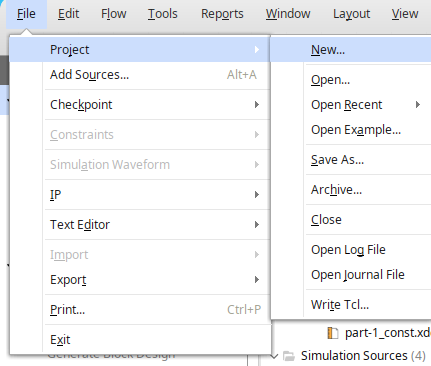
\includegraphics[width=0.5\textwidth]{figure_3_1.png}
%    \label{Figure 3.1}
%\end{figure}\newline

%\begin{center}
%    Truth Table 1: AND Gate Waveform
%    \begin{displaymath}
%    \begin{array}{|c c|c|}
%    In1 & In2 & In1 \land In2\\
%    \hline
%    F & F & F\\
%    F & T & F\\
%    T & F & F\\
%    T & T & T\\
%    \end{array}
%    \end{displaymath}
%\end{center}

\documentclass{article}
\usepackage{graphicx} % Required for inserting images
\usepackage{varwidth}

\title{Experiment 2 Lab Report \\ \large EEE3342C - 00012}
\author{Yousef Awad}
\date{January 2025}
\setcounter{secnumdepth}{0}

\begin{document}

\maketitle
\tableofcontents
\newpage

\section{Equipment}
For this experiment a computer running Linux 6.12.9 was used alongside the Xilinx Vivado 2024.2 software, alongside an FPGA board, the BASYS 3 development board. The board specifically only used to ensure the simulation by the Vivado software was accurate in the real world, as well as to verify the simulation software wasn't incorrect.
\section{Objective}
The objective for this lab was to explain and show how to create efficient test benches that are modular in nature ass well as the methodology via the creation and analysis of given Verilog testbenches. This was specifically done, so that it can easily be scaled to multiple input sizes for whatever circuit is made, as well as specific practical tasks such as 2 circuits below and via debugging a third.
\section{Part 2: Simple Boolean Network Testbench}
The circuit given for this part was the following:
$$ \neg[(A \land B) \lor \neg (C \lor D)] $$
Of which has the following given schematic:
\begin{figure}[!htbp]
    \centering
    \caption{}
    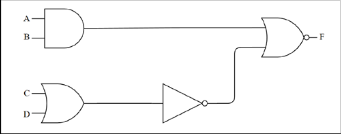
\includegraphics[width=0.5\textwidth]{part-2-schem.png}
    \label{Figure 1}
\end{figure}\newpage
And when compiled into a truth table with the inputs of A, B, C, D and an output of F, would be the following:
\begin{center}
    Truth Table
    \begin{displaymath}
    \begin{array}{| c  c  c  c |c|}
    A & B & C & D & F\\
    \hline
    F & F & F & F & 0 \\
    F & F & F & T & 1 \\
    F & F & T & F & 1 \\
    F & F & T & T & 1 \\
    F & T & F & F & 0 \\
    F & T & F & T & 1 \\
    F & T & T & F & 1 \\
    F & T & T & T & 1 \\
    T & F & F & F & 0 \\
    T & F & F & T & 1 \\
    T & F & T & F & 1 \\
    T & F & T & T & 1 \\
    T & T & F & F & 0 \\
    T & T & F & T & 0 \\
    T & T & T & F & 0 \\
    T & T & T & T & 0 \\
    \end{array}
    \end{displaymath}
\end{center}
And when written up in verilog, has the following text:
\begin{figure}[!htbp]
    \centering
    \begin{verbatim}
    module BOOL_NETWORK(
          input A, B, C, D,
          output F
      );
      wire andAB, orCD;

      assign andAB = A & B;
      assign orCD = (C | D);

      assign F = ~(andAB | (~orCD));
      
    endmodule
    \end{verbatim}
\end{figure}\newpage
And when tested, used the following testbench, after reading through part 1 of the experiment manual:
\begin{figure}[!htbp]
    \centering
    \begin{verbatim}
    module bool_tb();
        parameter NUMIN = 4;
        reg[NUMIN - 1:0] count;
        integer i;
        
        reg a, b, c, d;
        wire out;
        
        BOOL_NETWORK UUT(.A(a), .B(b), .C(c), .D(d), .OUT(out));
        
        initial begin
            count = 0; // setting count to 000
            for (i = 0; i < 2**NUMIN; i = i + 1)begin
                a = count[3];
                b = count[2];
                c = count[1];
                d = count[0];
                count = count + 1;
                #10;
            end
        end
        
    endmodule
    \end{verbatim}
\end{figure}\newline
And, when simulated to confirm the truth table above to be true or false, it gave out the following waveform:
\begin{figure}[!htbp]
    \centering
    \caption{}
    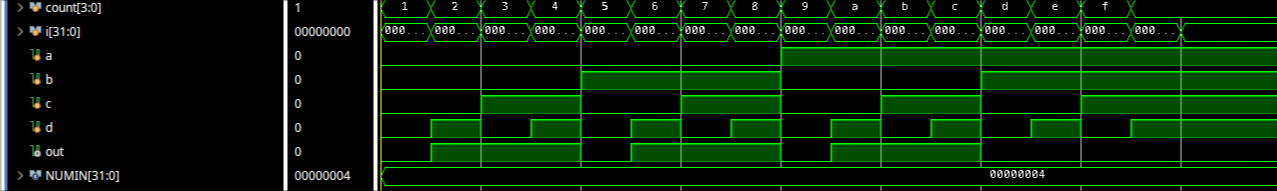
\includegraphics[width=1\textwidth]{part-2-wave.png}
    \label{Figure 2}
\end{figure}\newline
Of which perfectly shows that the truth table compiled above for the circuit is accurately shown in the simulation on Vivado. To ensure, even further, I then pushed the bitstream generated onto the BASYS board to manually enter and double check the simulation/truth table proper by flicking every possible combination.
\newpage
\section{Part 3: Complex Boolean Network Testbench}
The circuit given for this part was the following:
$$ [C \lor \neg(A \land B)] \oplus [\neg(D \lor E) \land \neg C] $$
Of which has the following given schematic:
\begin{figure}[!htbp]
    \centering
    \caption{}
    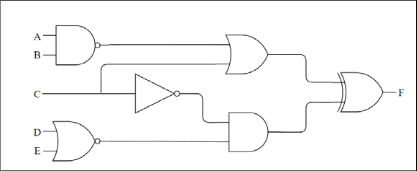
\includegraphics[width=0.5\textwidth]{part-3-schem.png}
    \label{Figure 1}
\end{figure}\newpage
And when compiled into a truth table with the inputs of A, B, C, D, E, and an output of F would be the following:
\begin{center}
    Truth Table
    \begin{displaymath}
    \begin{array}{| c  c  c  c  c | c |}
    A & B & C & D & E & F\\
    \hline
    F & F & F & F & F & 0 \\
    F & F & F & F & T & 1 \\
    F & F & F & T & F & 1 \\
    F & F & F & T & T & 1 \\
    F & F & T & F & F & 1 \\
    F & F & T & F & T & 1 \\
    F & F & T & T & F & 1 \\
    F & F & T & T & T & 1 \\
    F & T & F & F & F & 0 \\
    F & T & F & F & T & 1 \\
    F & T & F & T & F & 1 \\
    F & T & F & T & T & 1 \\
    F & T & T & F & F & 1 \\
    F & T & T & F & T & 1 \\
    F & T & T & T & F & 1 \\
    F & T & T & T & T & 1 \\
    T & F & F & F & F & 0 \\
    T & F & F & F & T & 1 \\
    T & F & F & T & F & 1 \\
    T & F & F & T & T & 1 \\
    T & F & T & F & F & 1 \\
    T & F & T & F & T & 1 \\
    T & F & T & T & F & 1 \\
    T & F & T & T & T & 1 \\
    T & T & F & F & F & 1 \\
    T & T & F & F & T & 0 \\
    T & T & F & T & F & 0 \\
    T & T & F & T & T & 0 \\
    T & T & T & F & F & 1 \\
    T & T & T & F & T & 1 \\
    T & T & T & T & F & 1 \\
    T & T & T & T & T & 1 \\
    \end{array}
    \end{displaymath}
\end{center}
And when written up in verilog, has the following text:
\begin{figure}[!htbp]
    \centering
    \begin{verbatim}
    module COMPLEX_BOOL_NETWORK(
            input A, B, C, D, E,
            output OUT // F
        );
        wire w1, w2, w3, w4;
        
        assign w1 = ~(A & B);
        assign w2 = ~(D | E);
        assign w3 = w1 | C;
        assign w4 = w2 & (~C);
        
        assign OUT = w3 ^ w4;
        
    endmodule
    \end{verbatim}
\end{figure}\newpage
And when tested, used the following testbench, after adapting the testbench from the last part (part 2):\\
\begin{figure}[!htbp]
    \centering
    \begin{verbatim}
    module complex_bool_tb();
        parameter NUMIN = 5;
        reg[NUMIN - 1:0] count;
        integer i;
        
        reg a, b, c, d, e;
        wire out; // F
        
        COMPLEX_BOOL_NETWORK UUT(.A(a), .B(b), .C(c), .D(d), .E(e), .OUT(out));
        
        initial begin
            count = 0;
            for (i = 0; i < 2**NUMIN; i = i + 1) begin
                a = count[4];
                b = count[3];
                c = count[2];
                d = count[1];
                e = count[0];
                
                count = count + 1;
                #10;
            end
        end
        
    endmodule
    \end{verbatim}
\end{figure}\newpage
And, when simulated to confirm the truth table above to be true or false, it gave out the following waveform:
\begin{figure}[!htbp]
    \centering
    \caption{}
    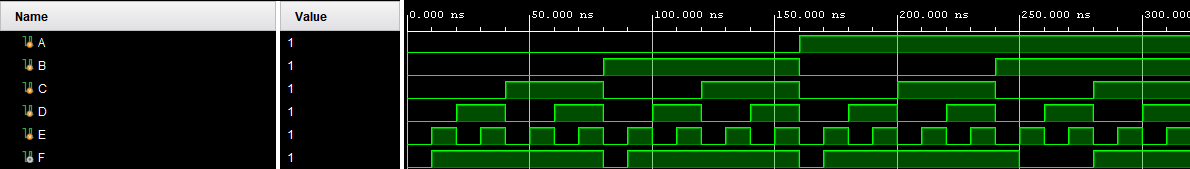
\includegraphics[width=1\textwidth]{part-3-wave.png}
    \label{Figure 2}
\end{figure}\newline
Of which perfectly shows that the truth table compiled above for the circuit is accurately shown in the simulation on Vivado. To ensure, even further, I then pushed the bitstream generated onto the BASYS board to manually enter and double check the simulation/truth table proper by flicking every possible combination.
\newpage
\section{Part 4: Application for Circuit Debugging}
In this part, we were given a faulty RTL code below, with them stating that w1, w2, and w3 are valid and true while the assign statements for X and Y are faulty.
\begin{figure}[!htbp]
    \centering
    \begin{verbatim}
    module logic_top(
            input A, B, C,
            output X, Y
        );
        wire w1, w2, w3;

        assign w1 = A ^ B;
        assign w2 = C & w1;
        assign w3 = A & B;

        assign X = C | w1;
        assign Y = w2 & w3;
    endmodule
    \end{verbatim}
\end{figure}\newline
As well as given the following truth table for the expected/wanted outputs of X and Y:
\begin{center}
    \begin{displaymath}
    \begin{array}{|c c c|c c|}
      A & B & C & X & Y\\
    \hline
      F & F & F & F & F\\
      F & F & T & T & F\\
      F & T & F & T & F\\
      F & T & T & F & T\\
      T & F & F & T & F\\
      T & F & T & F & T\\
      T & T & F & F & T\\
      T & T & T & T & T\\
    \end{array}
    \end{displaymath}
\end{center}
Now, to find out what the solutions for X and Y are, I proceeded to try and find out the truth table for w1, w2, and w3, as listed below:
\begin{center}
    \begin{displaymath}
    \begin{array}{|c c c|c c c|}
      A & B & C & w1 & w2 & w3\\
    \hline
      F & F & F & F & F & F\\
      F & F & T & F & F & F\\
      F & T & F & T & F & F\\
      F & T & T & T & T & F\\
      T & F & F & T & F & F\\
      T & F & T & T & F & F\\
      T & T & F & F & F & T\\
      T & T & T & F & F & T\\
    \end{array}
    \end{displaymath}
\end{center}
When analyzing this table, and comparing it to the X and Y table above it, I then deduced that the answer to the assignment of X and Y are the following:
\begin{figure}[!htbp]
    \centering
    \begin{verbatim}
    assign X = C ^ w1;
    assign Y = w2 | w3;
    \end{verbatim}
\end{figure}\newline
And when tested with the following testbench I made, it generated the following waveform, correctly showing the waveform/truth table wanted.
\begin{figure}[!htbp]
    \centering
    \begin{verbatim}
    module circuit_debugging_tb();
        parameter NUMIN = 3;
        reg[NUMIN - 1:0] count;
        integer i;
        
        reg a, b , c; // inputs are registers
        wire x, y; // wires are outputs
        
        CIRCUIT_DEBUGGING UUT(.A(a), .B(b), .C(c), .X(x), .Y(y));
        
        initial begin
            count = 0;
            for (i = 0; i < 2**NUMIN; i = i + 1) begin
                a = count[2];
                b = count[1];
                c = count[0];
                
                count = count + 1;
                #10;
            end
        end
        
    endmodule
    \end{verbatim}
\end{figure}\newline
\begin{figure}[!htbp]
    \centering
    \caption{}
    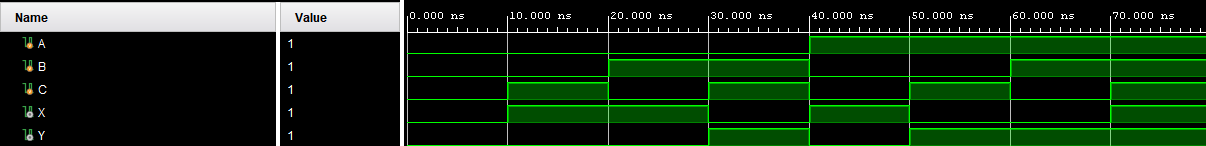
\includegraphics[width=1\textwidth]{part-4-wave.png}
\end{figure}\newpage
And, for reference, can be compared to the waveform before the change:
\begin{figure}[!htbp]
    \centering
    \caption{}
    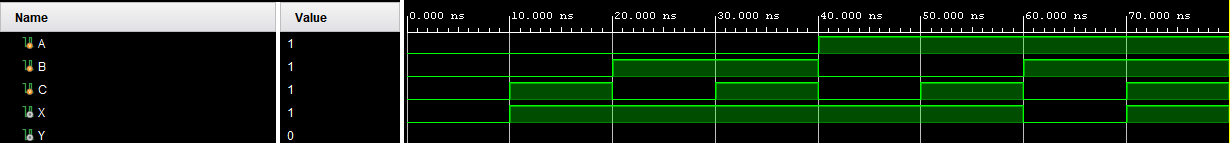
\includegraphics[width=1\textwidth]{part-4-wave-before.png}
\end{figure}\newline
As well as generated the following schematic and boolean algebra equation proper:
\begin{figure}[!htbp]
    \centering
    \caption{}
    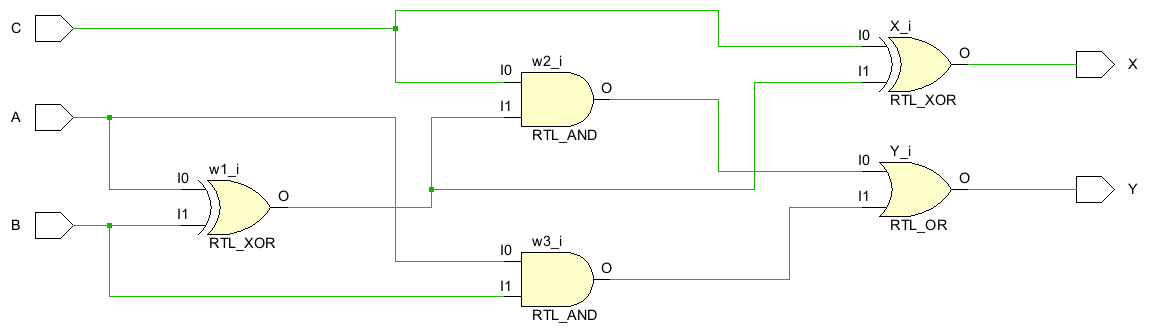
\includegraphics[width=1\textwidth]{part-4-schem.png}
\end{figure}\newline
$$ X = C \oplus (A \oplus B) $$
$$ Y = [C \land (A \oplus B)] \land (A \land B) $$
\newline
\section{Conclusion}
This experiment refined as well as explained further how testbenches work, as well as their importance in why testing circuits is important to ensure functionality. Alongside this, it practically improved my skills in writing RTL as well as debugging via truth tables, so as to ensure a proper output is designed.
\end{document}
